% This must be in the first 5 lines to tell arXiv to use pdfLaTeX, which is strongly recommended.
\pdfoutput=1
% In particular, the hyperref package requires pdfLaTeX in order to break URLs across lines.

\documentclass[11pt]{article}

% Remove the "review" option to generate the final version.
\usepackage[]{ACL2023}

% Standard package includes
\usepackage{times}
\usepackage{latexsym}

% For proper rendering and hyphenation of words containing Latin characters (including in bib files)
\usepackage[T1]{fontenc}
% For Vietnamese characters
% \usepackage[T5]{fontenc}
% See https://www.latex-project.org/help/documentation/encguide.pdf for other character sets

% This assumes your files are encoded as UTF8
\usepackage[utf8]{inputenc}

% This is not strictly necessary, and may be commented out.
% However, it will improve the layout of the manuscript,
% and will typically save some space.
\usepackage{microtype}

% This is also not strictly necessary, and may be commented out.
% However, it will improve the aesthetics of text in
% the typewriter font.
\usepackage{inconsolata}

\usepackage{graphicx}


% If the title and author information does not fit in the area allocated, uncomment the following
%
%\setlength\titlebox{<dim>}
%
% and set <dim> to something 5cm or larger.

\title{Extractive summarisation of biomedical research articles using TextRank, WordRank, and a hybrid approach}

% Author information can be set in various styles:
% For several authors from the same institution:
% \author{Author 1 \and ... \and Author n \\
%         Address line \\ ... \\ Address line}
% if the names do not fit well on one line use
%         Author 1 \\ {\bf Author 2} \\ ... \\ {\bf Author n} \\
% For authors from different institutions:
% \author{Author 1 \\ Address line \\  ... \\ Address line
%         \And  ... \And
%         Author n \\ Address line \\ ... \\ Address line}
% To start a seperate ``row'' of authors use \AND, as in
% \author{Author 1 \\ Address line \\  ... \\ Address line
%         \AND
%         Author 2 \\ Address line \\ ... \\ Address line \And
%         Author 3 \\ Address line \\ ... \\ Address line}

\author{Kristina Levina \\
  Linköping University, STIMA \\
  Course code: 732A81 \\
 \texttt{krile102} \\}

\begin{document}
\maketitle
\begin{abstract}
This project aims at building a tool to generate a summary of a biomedical research manuscript automatically based on the main text. To this end, extractive summarisation is employed. The motivation behind choosing extractive summarisation is, in essense, the neccessety to preserve key sentences from the main text. Extractive summarisation will retrieve sentences based on their importance without rephrasing them, thereby excluding misinterpretations. The meaning preservation is crucial for scientific texts. In this project, PubMed dataset is used. A subset of 100 articles and their abstracts have been manually looked through and filtered so that articles and abstracts have similar characteristincs in terms of relative number of sentences of the abstract to the main text. As a result, 24 articles and their human-written summaries (abstracts) were selected. Three algorithms were chosen for extractive summarisation: TextRank, WordRank, and their combination. Their performance was assessed using ROUGE (recall), BLEU (precision), and F1 score. The obtained results show that Y better suits for the considered task. 

\end{abstract}

\section{Introduction}

With increasing volume of published articles in medical research, it becomes increasingly difficult for doctors, medical staff, and public health officials to stay updated. Sometimes, a

\section{Theory}
\subsection{PageRank}

The Google PageRank algorithm is explained in \citet{rogers2002google}. This algorithm allows to determine the importance of a web page. This is crucial for search engine optimisation. The PageRank of page $A$ is calculated as follows:

\begin{small}
\begin{equation}
 PR(A) = (1-d) + d \left(\frac{PR(T1)}{C(T1)} + ... + \frac{PR(Tn)}{C(Tn)}\right),
 \label{eq:pr}
\end{equation}
\end{small}
where $PR$ denotes PageRank; $d$ denotes a damping factor, which can be set between 0 and 1; pages $T1...Tn$ link to $A$; and $C(A)$ denotes the number of links going out of page $A$. The calculation is straightforward once $PR(T1)...PR(Tn)$ are known, but they are not. To exclude excessive influence of pages $T1..Tn$, the factor $d$ is set to 0.85 according to \citet{rogers2002google}. Terms $1-d$ are added so that $PR(A)$ is a probability distribution representing likelihood that a person randomly clicking on links will arrive at any particular page (sum of all pages' PageRanks will be one).

The recursive nature of Eq. (\ref{eq:pr}) means that one cannot determine $PR(A)$ without knowing $PR(T1)...PR(Tn)$. If a circular linking is introduced, this becomes cumbersome. However, initial parameters (PageRanks) can be set, and the calculation can be performed iteratively until convergence. This procedure can be computationally intensive if a large number of pages and links is involved. The resulting distribution would be close to the real probability distribution if not stacked in local minimum. Various optimisation techniques of PageRank algorithm have been proposed, including particle swarm optimisation (\citet{bastos2021inverse}).  An illustration of the PageRank algorithm is shown in Fig. \ref{fig:PR}.

\begin{figure}[!h]
\centering
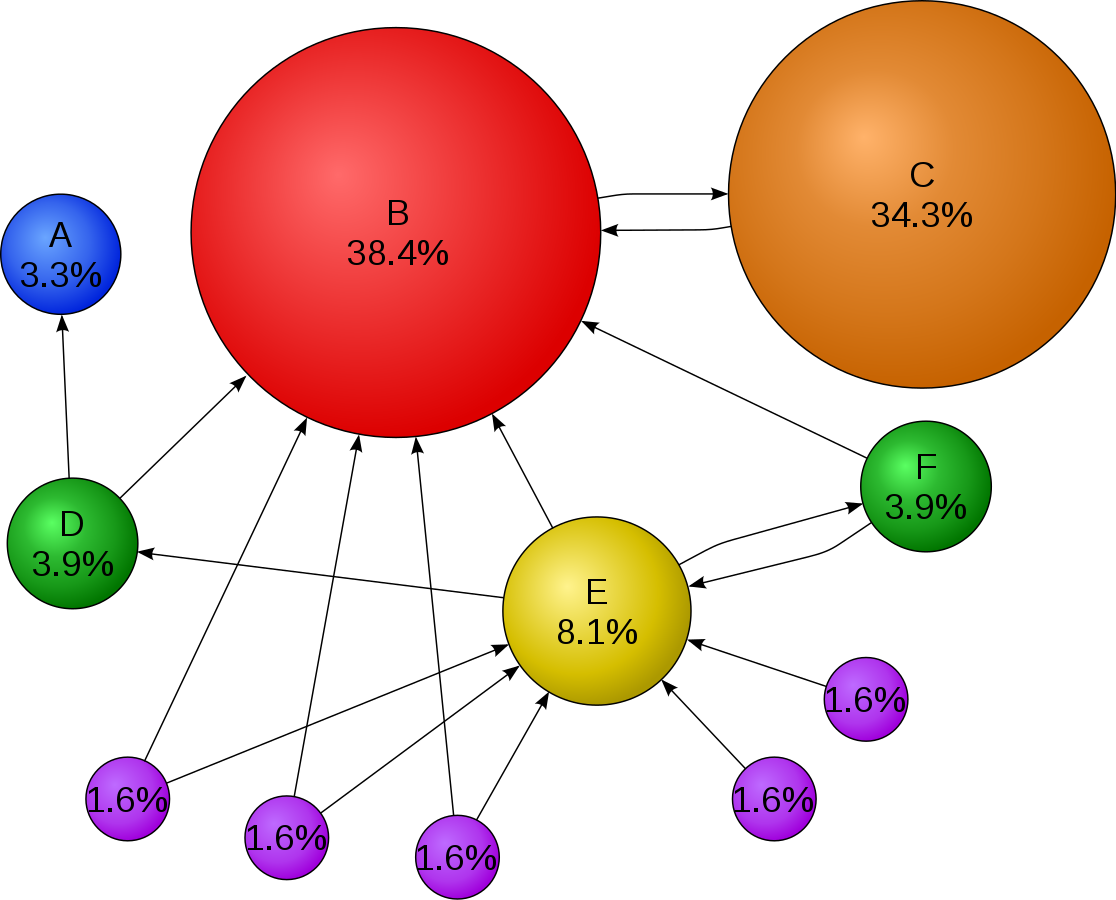
\includegraphics[scale = 0.175]{../figures/PR.png}
\caption{Figure source: \href{https://en.wikipedia.org/wiki/File:PageRanks-Example.svg}{Wikipedia}. Illustration of the PageRank algorithm. The percentage shows the perceived importance, and the arrows represent hyperlinks.\label{fig:PR}}
\end{figure}

\subsection{TextRank}
\label{subsect:textrank}

TextRank algorithm has been introduced by \citet{mihalcea2004textrank}. This is an unsupervised method of extractive summarisation. Sentences are ranked based on their similarity scores to each other. First, sentences are vectorised. Second, a similarity matrix between sentence vectors is computed. A graph is constructed such that sentences are nodes and similarity scores are edges. The PageRank algorithm is then run with sentences treated as pages and similarity scores as links. This simple idea enables to extract most important sentences (top ranked) from a text. The top sentence in the list will be that having the highest similarity to all other sentences in the text. In other words, the top extracted sentence will be related to most of other sentences in the text. A flowchart of WordRank is shown in Fig. \ref{fig:textrank}

\begin{figure}[!h]
\centering
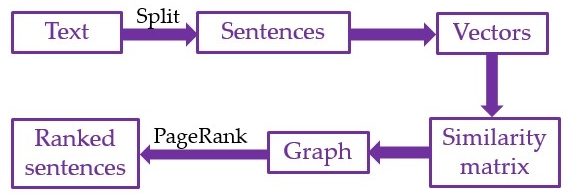
\includegraphics[scale = 0.5]{../figures/textrank.jpg}
\caption{Flowchart of TextRank.\label{fig:textrank}}
\end{figure}

\subsection{WordRank}
\label{subsect:wordrank}

WordRank is a modified version of TextRank \citep{reza2020}. The initial text is split into words. First, the words are vectorised. Second, a similarity matrix between word vectors is computed. A graph is constructed such that words are nodes and similarity scores are edges. The PageRank algorithm is then run with words treated as pages and similarity scores as links. Finally, the score of a sentence is the sum of the scores of all the words in that sentence. Top scored sentences are used for generating summary. A flowchart of WordRank is shown in Fig. \ref{fig:wordrank}

\begin{figure}[!h]
\centering
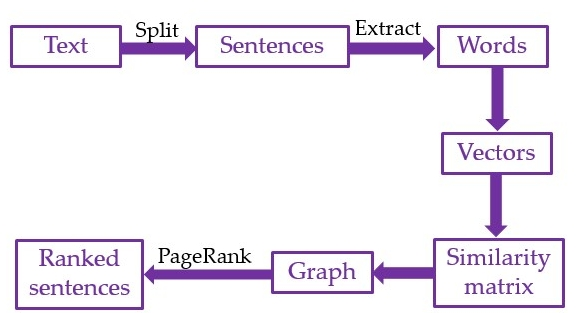
\includegraphics[scale = 0.5]{../figures/wordrank.jpg}
\caption{Flowchart of WordRank.\label{fig:wordrank}}
\end{figure}

\subsection{BERTSUM}

Bidirectional Encoder Representations from Transformers (BERT) is a family of masked-language models published in 2018 by Google \citep{devlin2019google}. The BERT architecture and operation principle is explained by \citet{rogers2021primer}. Citing them ``Fundamentally, BERT is a stack of Transformer encoder layers that consist of multiple self-attention “heads”. For every input token in a sequence, each head computes key, value, and query vectors, used to create a weighted representation. The outputs of all heads in the same layer are combined and run through a fully connected layer. Each layer is wrapped with a skip connection and followed by layer normalization.''

The use of BERT for extractive summarisation is outlined by \citet{liu2019text}. The authors modified the BERT architecture (BERTSUM) for extractive text summarisation. Both architectures are shown in Fig. \ref{fig:bert}


\begin{figure*}[!h]
\centering
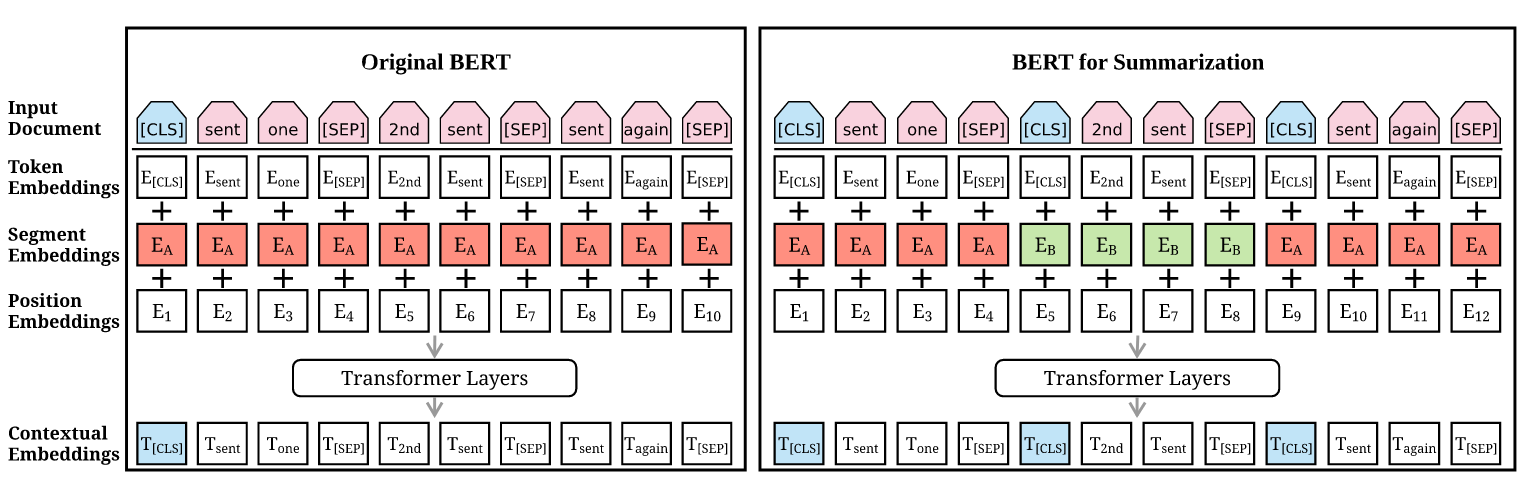
\includegraphics[scale = 0.4]{../figures/bert.png}
\caption{Figure source: \citet{liu2019text}.Architecture of the original BERT model (left) and BERTSUM (right). The input document is a sequence on top. It is followed by the summation of three types of embeddings for each token. The summed vectors are used
as input embeddings to several bidirectional Transformer layers, generating contextual vectors for each token. BERTSUM extends BERT by inserting multiple [CLS] symbols to learn sentence representations and using interval segmentation embeddings (illustrated in red and green color) to distinguish multiple sentences.\label{fig:bert}}
\end{figure*}


\subsection{Evaluation metrics}

How to compare human-generated summaries with machine-generated summaries? One can compare the occurrence of n-grams \citep{lin2003automatic} in both texts in terms of both precision and recall. In the context of comparison of a human-generated text with a machine-generated text, the recall metric is called ROUGE \citep{lin2003automatic}, and the precision metric is called BLEU \citep{papineni2002bleu}). 

ROUGE and BLEU are complementing evaluation metrics. If many n-grams from a machine-generated summary appear in a human-generated summary, BLEU is high, and if many n-grams from a human-generated summary appear in a machine-generated summary, ROUGE is high.

F1 score is a harmonic mean between ROUGE and BLEU:
\begin{equation}
 F1 = \frac{2\cdot BLEU \cdot ROUGE}{BLEU + ROUGE},
 \label{eq:f1}
\end{equation}
being a good performance indication metric overall.

One has to be aware of brevity penalty, when calculating BLEU. Consider the following example of a machine generated summary: \begin{verbatim}the the the the\end{verbatim} and a human-generated summary: \begin{verbatim}the cat likes mice\end{verbatim} The BLEU metric will be $4/4 = 1$ (aka four words from the machine-generated summary appear in the human-generated summary). However, the machine-generated summary is poor. To fix this, a brevity penalty is introduced: the repetition number of a word to take into account in BLEU can be as high as the repetition number of the word in the human-generated summary. In the example above, \texttt{the} appears only once in the machine-generated summary. Thus, BLEU is $1/4=0.25$, reflecting the poor quality of the machine-generated summary.

\section{Data}
\label{sect:data}

Data are taken from the paper by \citet{cohan2018discourse}. This dataset contains a large collection (100,000) of scientific articles from the biomedical domain (OpenAccess PubMed articles). Data are hosted in \href{https://github.com/armancohan/long-summarization}{GitHub}. Each article has the following fields: 
\begin{verbatim}
{ 
  'article_id': str,
  'abstract_text': List[str],
  'article_text': List[str],
  'section_names': List[str],
  'sections': List[List[str]]
}
\end{verbatim}

For this project, I have looked through 100 articles and considered only articles meeting the following assumptions: First, the provided abstract should be between 8\%--12\% of the main text in terms of number of sentences. This is to ensure similar conditions for generating summaries. Second, the number of sentences of the main manuscript text should be larger than 50 to meet the objective of long document summarisation. Out of 100 articles, only 24 met this conditions.

An example of the beginning of one chosen article is as follows:

\texttt{'["anxiety affects quality of life in those living with parkinson \'s disease ( pd ) more so than overall cognitive status , motor deficits , apathy , and depression [ 13 ] .", \'although anxiety and depression are often related and coexist in pd patients , recent research suggests that anxiety rather than depression is the most prominent and prevalent mood disorder in pd [ 5 , 6 ] . yet ,\', }

The beginning of the corresponding summary is as follows:

\texttt{'["<S> research on the implications of anxiety in parkinson \'s disease ( pd ) has been neglected despite its prevalence in nearly 50\% of patients and its negative impact on quality of life . </S>", \'<S> previous reports have noted that neuropsychiatric symptoms impair cognitive performance in pd patients }

The data have been already tokenised. From the abstract text, <S> and </S> tags were removed. Further preprocessing included stop word removal, lemmatisation, and non-alphabetic characters' removal. This preprocessing has been done using the Spacy language model. Stop words were removed to avoid sentence ranking based on common and frequent words rather than important words. Lemmatisation was used to treat same words in an exactly same manner. Non-alphabetic characters were removed to avoid their influence on the ranking results. Punctuation and numerals should not affect the sentence importance.
 

\section{Method}

After data pre-processing explained in Sect. \ref{sect:data}, the initial text was split into a list of sentences (see function \texttt{preprocess} in the \texttt{main\_project.py} file). All the methods explained below yielded as many sentences as was in the corresponding human-written summary to ensure equal evaluation conditions.´                                                                                                                                        
                                                                                                                                          
\subsection{TextRank}

Following the procedure outlined in Sect. \ref{subsect:textrank}, a list of preprocessed sentences was input into \texttt{textrank} function (see \texttt{main\_project.py} file). Then the sentences were vectorised as bags of words using word embeddings from \texttt{Spacy}:

\begin{equation}
 vect(sent) = \sum_{i = 1}^N (embed(word_i)),
\end{equation}
where $word_i$ is a word of a sentence $sent$, $N$ is the number of all words in the sentence, and $embed(word_i)$ is the \texttt{Spacy} embedding of $word_i$.

The cosine similarity was then used to compute the similarity between the vectors of all sentences. The obtained similarity scores were used to construct a similarity matrix. The obtained similarity matrix was transformed into a graph using Python library \texttt{nx}. PageRank was run using \texttt{nx.pagerank}. The sorted sentence scores were outputted from the function \texttt{textrank}.

\subsection{WordRank}

Following the procedure outlined in Sect. \ref{subsect:wordrank}, a list of preprocessed sentences was input into \texttt{wordrank} function (see \texttt{main\_project.py} file). Herein, the words were embedded using \texttt{Spacy} embeddings. The cosine similarity was again used to compute similarity scores between word vectors. The obtained similarity scores were used to construct a similarity matrix. The obtained similarity matrix was transformed into a graph using Python library \texttt{nx}. PageRank was run using \texttt{nx.pagerank}. The sentence score was found as the summation of the scores of all words in the sentence. The sorted sentence scores were outputted from the function \texttt{textrank}.

\subsection{Hybrid}

The TextRank algorithm is bound to favour longer sentences, resulting in high BLEU score. In contrast, the WordRank algorithm favours sentences with the most related words to other words, resulting in high ROUGE. This idea is outlined by \citet{reza2020}. Could this two algorithms be combined so that the F1 score is higher than that of individual algorithms? \citet{reza2020} used a combination of WordRank and TextRank. First, WordRank was run to extract 64\% of the initial sentences. The TextRank was then run on these 64\% extracted sentences to obtain 8\% of the initial text as a generated summary. This combination worked best in \citet{reza2020}. 

Here, their experiment is repeated. In addition, a hybrid algorithm with WordRank extracting 80\% of the initial text and TextRank extracting the required number of sentences was run. The relevant code is found in functions \texttt{hybrid64} and \texttt{hybrid80} in the \texttt{main\_project.py} file.

\subsection{BERTSUM}

The BERTSUM was run on the preprocessed initial texts on Google Colab using the library \texttt{bert-extractive-summarizer}.

\subsection{Evaluation}

The human-written summaries and the machine-generated summaries were split into unigrams, bigrams, and trigrams. Subsequently, BLEU, ROUGE, and F1 scores were obtained. The brevity factor was taken into the account. (See function \texttt{evaluation\_report} in the \texttt{main\_project.py} file)

After all 24 experiments, the obtained BLEU, ROUGE, and F1 scores were averaged, and their mean (e.g. $\overline{F1}$) and standard deviation (e.g. $\sigma(F1)$) values were obtained. The corresponding margins of error (95\%confidence) were computed following the usual frequentist approach:

\begin{equation}
 F1 = \overline{F1} \pm 1.96 \frac{\sigma(F1)}{\sqrt(24)}.
\end{equation}


\section{Results}

The ROUGE\_1, BLEU\_1, and F1\_1 scores respectively denote ROUGE, BLEU, and F1 scores of unigrams between the human-written and generated summaries. The results are shown in Fig. \ref{fig:uni} and Tables \ref{tab:means} and \ref{tab:mors}. TextRank (36.0), Hybrid64 (35.7) and Hybrid80 (35.9) yield high mean F1\_1 scores relative to WordRank (30.3), but considering margin of error, the estimation by Hybrid80 is slightly more robust (35.9 $\pm$ 3.3 versus 36.0 $\pm$ 3.7). The highest mean F1\_1 score shows BERTSUM (37.7 $\pm$ 3.9). TextRank (27.0 $\pm$ 3.7), Hybrid64 (26.7 $\pm$ 3.1), and Hybrid80 (26.8 $\pm$ 3.2) yield high mean BLEU\_1 scores relative to WordRank (20.8 $\pm$ 3.2). The highest BLEU\_1 value shows BERTSUM (30.4 $\pm$ 3.7). WordRank yields the highest ROUGE\_1 score (60.1 $\pm$ 4.1) in comparison to other algorithms. The lowest ROUGE\_1 score belongs to BERTSUM (51.2 $\pm$ 5.0).

The ROUGE\_2, BLEU\_2, and F1\_2 scores respectively denote the ROUGE, BLEU, and F1 scores of bigrams between the human-written and generated summaries. The results are shown in Fig. \ref{fig:bi} and Tables \ref{tab:means} and \ref{tab:mors}. The ROUGE\_3, BLEU\_3, and F1\_3 scores respectively denote the ROUGE, BLEU, and F1 scores of trigrams between the human-written and generated summaries. The results are shown in Fig. \ref{fig:tri} and Tables \ref{tab:means} and \ref{tab:mors}. TextRank shows the highest values of ROUGE\_2 and ROUGE\_3 (21.2 $\pm$ 4.9 and 10 $\pm$ 3.7, respectively) and F1\_2 and F1\_3 (13.4 $\pm$ 3.2 and 6.5 $\pm$ 2.5, respectively). However, regarding BLEU\_2, BERTSUM (10.3 $\pm$ 2.9) yields slightly higher mean value than TextRank (10.1 $\pm$ 2.7). 

The total running times of all four algorithms for summarisation of 24 data samples is shown in Table \ref{tab:time}. TextRank (1 min) performs 16 times faster than WordRank, Hybrid64, and Hybrid80 algorithms (16 min). BERTSUM (24 min) runs very slowly in comparison to TextRank.

\begin{figure}[!h]
\centering
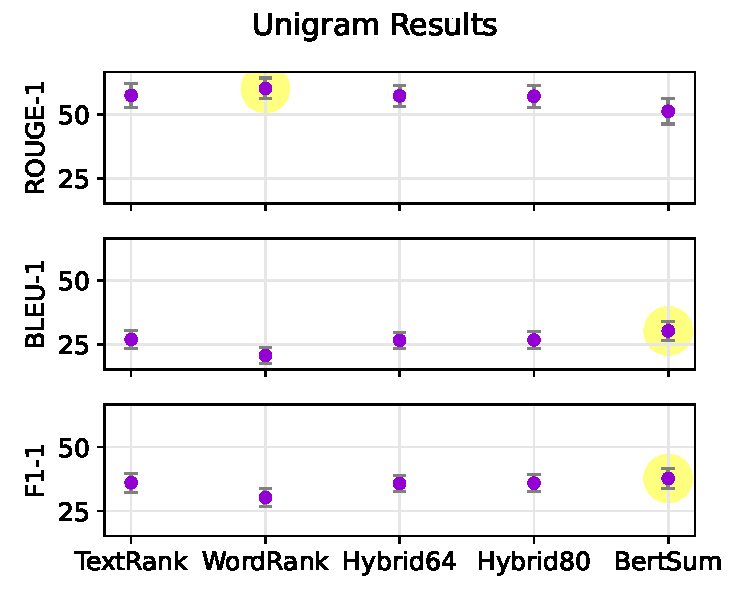
\includegraphics[scale = 0.5]{../figures/unigrams.pdf}
\caption{ROUGE, BLEU, and F1 score of unigrams between the human-written and generated summaries.\label{fig:uni}}
\end{figure}

\begin{figure}[!h]
\centering
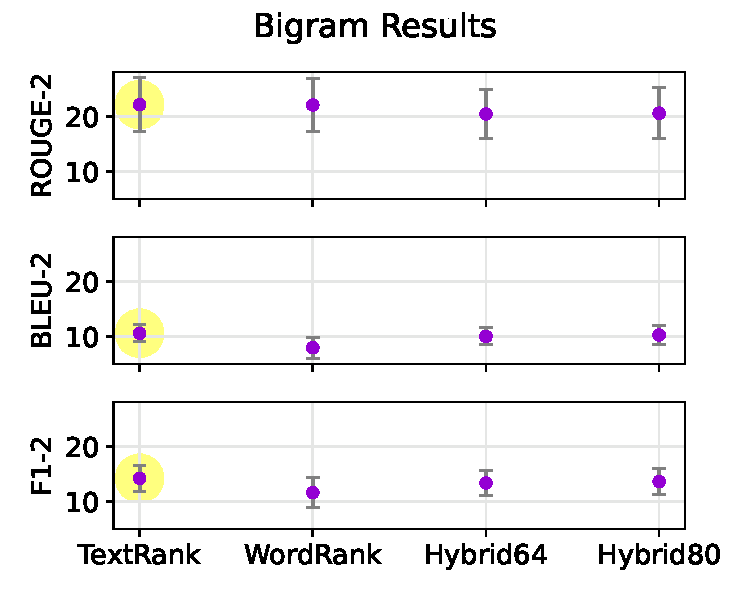
\includegraphics[scale = 0.5]{../figures/bigrams.pdf}
\caption{ROUGE, BLEU, and F1 score of bigrams between the human-written and generated summaries.\label{fig:bi}}
\end{figure}

\begin{figure}[!h]
\centering
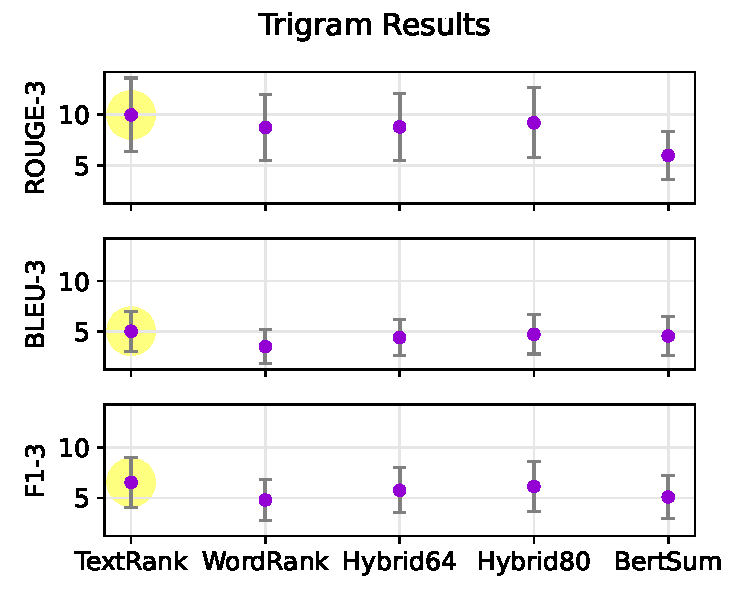
\includegraphics[scale = 0.5]{../figures/trigrams.pdf}
\caption{ROUGE, BLEU, and F1 score of trigrams between the human-written and generated summaries.\label{fig:tri}}
\end{figure}

\begin{table*}[!h]
\centering
\begin{tabular}{l|lllll}
\hline
&\textbf{TextRank} & \textbf{WordRank} & \textbf{Hybrid64} & \textbf{Hybrid80} & \textbf{BERTSUM}\\
\hline
ROUGE\_1 & 57.4 & \textbf{60.1} & 57.2 & 57.1& 51.2\\
ROUGE\_2 & \textbf{21.2} & 20.3 & 19.9 & 20.3& 16.0\\
ROUGE\_3 & \textbf{10.0} & 8.7 & 8.8 & 9.2& 6.0\\
BLEU\_1 & 27.0 & 20.8 & 26.7 & 26.8& \textbf{30.4}\\
BLEU\_2 & 10.1 & 7.3 & 9.5 & 9.8& \textbf{10.3}\\
BLEU\_3 & \textbf{5.0} & 3.5 & 4.4 & 4.7& 4.6\\
F1\_1 & 36.0 & 30.3 & 35.7 & 35.9& \textbf{37.7}\\
F1\_2 & \textbf{13.4} & 10.4 & 12.6 & 12.9& 12.3\\
F1\_3  & \textbf{6.5} & 4.8 & 5.8 & 6.1& 5.1\\
\hline
\end{tabular}

\caption{\label{tab:means}
Mean values of the ROUGE, BLEU, and F1 metrics for unigrams, bigrams, and trigrams yielded by TextRank, WordRank, Hybrid64, Hybrid80, and BERTSUM methods.
}
\end{table*}

\begin{table*}[!h]
\centering
\begin{tabular}{l|lllll}
\hline
&\textbf{TextRank} & \textbf{WordRank} & \textbf{Hybrid64} & \textbf{Hybrid80} & \textbf{BERTSUM}\\
\hline
ROUGE\_1 & 4.7 & 4.1 & 4.1 & 4.3 & 5.0\\
ROUGE\_2 & 4.9 & 4.6 & 4.4 & 4.7 & 4.0\\
ROUGE\_3 & 3.7 & 3.2 & 3.3 & 3.5 & 2.4\\
BLEU\_1 & 3.7 & 3.2 & 3.1 & 3.2 & 3.7\\
BLEU\_2 & 2.7 & 2.2 & 2.3 & 2.5 & 2.9\\
BLEU\_3 & 2.0 & 1.7 & 1.8 & 1.9 & 2.0\\
F1\_1 &  3.7 & 3.6 & 3.2 & 3.3 & 3.9\\
F1\_2 & 3.2 & 2.8 & 2.9 & 3.1 & 3.2\\
F1\_3  & 2.5 & 2.0 & 2.2 & 2.4 & 2.1\\
\hline
\end{tabular}
\caption{\label{tab:mors}
Margins of error values of the ROUGE, BLEU, and F1 metrics for unigrams, bigrams, and trigrams yielded by TextRank, WordRank, Hybrid64, Hybrid80, and BERTSUM methods.
}
\end{table*}


\begin{table*}[!h]
\centering
\begin{tabular}{l|lllll}
\hline
&\textbf{TextRank} & \textbf{WordRank} & \textbf{Hybrid64} & \textbf{Hybrid80} & \textbf{BERTSUM}\\
\hline
Running time (min) & 1 & 16 & 16 & 16 & 24\\
\hline
\end{tabular}
\caption{\label{tab:time}
Running time (min) of all five algorithms considered in this project.
}
\end{table*}

\subsection{Example Result -- include if time -- if not -- limitation}

\section{Discussion}

\section{Conclusion}



% Entries for the entire Anthology, followed by custom entries
\bibliography{custom}
\bibliographystyle{acl_natbib}


\end{document}
